%!TEX root = main.tex
\chapter{Methods}
\label{chap:methods}

In this section we will outline which methods we have used for conducting the work.
\section{Data preparation}

When we got the dataset it was stored in three folders, one for each month (9, 10, 11) and within each folder were multiple chunks of data in Apache Avro format\cite{apacheavro} which we learned is a format similar to JSON and easily convertible. The chunks were contained in folders bearing the number for each month, however they were sorted by when the server had received the data packet containing the location from the phone and not when the phone had registered the location. The app is storing the collected data on the users phone for a maximum of one month, if the data is not uploaded within a month it is discarded. This approach to data collection means the month folders can contain location updates from the previous month as well.

\subsection{Preparation of Test data}
In this section we will demonstrate what we have done to prepare the test data.

\subsubsection{Data import to database}
We converted the Apache Avro formatted files to JSON format and imported them to a PostgreSQL database which allowed us to easily manipulate the data using SQL. We created a single table with the schema shown in Table \ref{table:schema_denormalized}. We decided to compute the time and spatial bins on insertion, thus we only had to compute them once. We created indexes on the following features: \textit{start\_time}, \textit{end\_time}, \textit{location}, \textit{useruuid}, \textit{spatial\_bin}, \textit{time\_bins}, \textit{country}.
Initially we created a normalized database with several relations. We discovered however that a deonormalized database might improve our performance, as we reduce the number of tables and and thus the number of joins required\cite{sanders2001denormalization}. The interaction with the data consists mostly of data extraction, after the initial insertion of the data and after removing all relations our performance improved significantly.

\begin{table}[htbp]
\centering

\begin{tabular}{|c|c|c|c|c|c|c|c|c|c|c|}
\hline
\textbf{Field name} & \textbf{Field type}    \\
\hline
id                  & SERIAL PRIMARY KEY     \\
\hline
useruuid            & TEXT NOT NULL          \\
\hline
start\_time         & TIMESTAMPTZ NOT NULL   \\
\hline
end\_time           & TIMESTAMPTZ NOT NULL   \\
\hline
location            & GEOGRAPHY(POINT, 4326) \\
\hline
altitude            & INTEGER NOT NULL       \\
\hline
accuracy            & INTEGER NOT NULL       \\
\hline
region              & TEXT                   \\
\hline
country             & TEXT                   \\
\hline
area                & TEXT                   \\
\hline
place               & TEXT                   \\
\hline
time\_bins          & INTEGER{[}{]} NOT NULL \\
\hline
spatial\_bin        & BIGINT NOT NULL        \\
\hline
\end{tabular}
\caption{Denormalized database schema}
\label{table:schema_denormalized}
\end{table}

\subsubsection{Binning} \label{ssec:binning}
In the following section the term grid cell or spatial bin will be used synonymously, the same holds for time interval and time bin.
A spatiotemporal co-occurrence between two users is defined as an instance in which they co-occurred in approximately the same time and approximately the same place.
We have partitioned or binned the globe into a discrete grid where the cells span .001{\degree} of latitude and longitude on each side (approximately 111m at the equator), and in a discrete time interval of 1-hour.
Thus we say a co-occurrence happens between users $i$ and $j$ if they share the same .001{\degree} spatial cell C within the same discrete time interval. We chose 0.001 as bin size as the location updates from GPS allowed for a high resolution.

Each grid cell has a unique ID, this is obtained by considering the grid as a matrix and flattening it to a list by traversing from left to right and top to bottom (row-first ordering) and using the list index as an ID. This makes a total possible spatial bin indexes of: $$(190 \cdot d)\cdot(360\cdot d)$$ where $d$ is the number of decimals. This makes in our case a total number of spatial bins of $68.400.000.000$ with our case of $d=3$.

We calculated the time bins by counting every hour from the start of the day of the earliest date appearing in the dataset, which has the ISO 8601 timestring: "2015-08-09 22:25:33.766+02". The last day has the ISO 8601 timestring: "2015-12-01 00:59:15.738+01". This leaves us with $2738$ possible time bin IDs. As each location update has a start\_time and an end\_time, each update will result in one or more entries for each time bin dependent on the duration between start\_time and end\_time. \textcolor{red}{We chose a time bin size of 1 hour as the location updates between users were sparse, DISKUTER MED ANDERS}  For generating our dataset we count co-occurrences between dyads only once per distinct spatial and time bin, as duplicates would result in an artificially inflated number of co-occurrences between dyads.
\begin{figure}[H]
    \hspace*{-1.0cm}
    \centering
    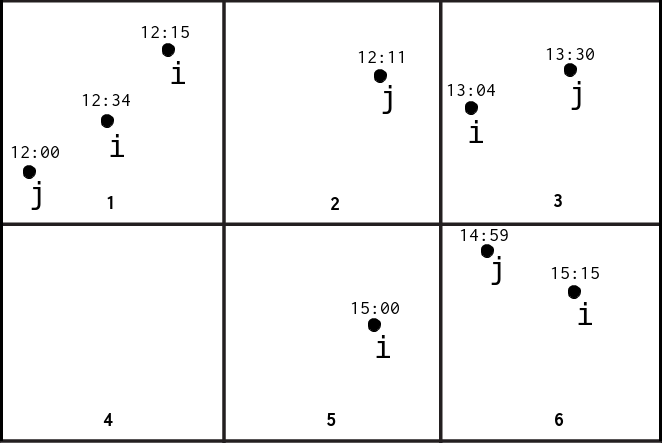
\includegraphics[scale=0.30]{grid}
    \caption{Illustration of spatiotemporal co-occurrences, users $i$ and $j$ have 2 co-occurrences in spatial bin 1 and 3, the users in spatial bin 6 have different time bins.}
    \label{fig:binning}
\end{figure}

\subsubsection{Visualization}
We used \textit{Basemap}\cite{basemap}, for plotting static visualizations of all the locations at once and \textit{Leaflet}\cite{leaflet} for producing interactive maps to visualize the data. We created a map for visualizing the users location traces over time and we created one that allowed us to see all the co-occurrences that happened between a pair of users.
\begin{figure}[H]
    \hspace*{-1.0cm}
    \centering
    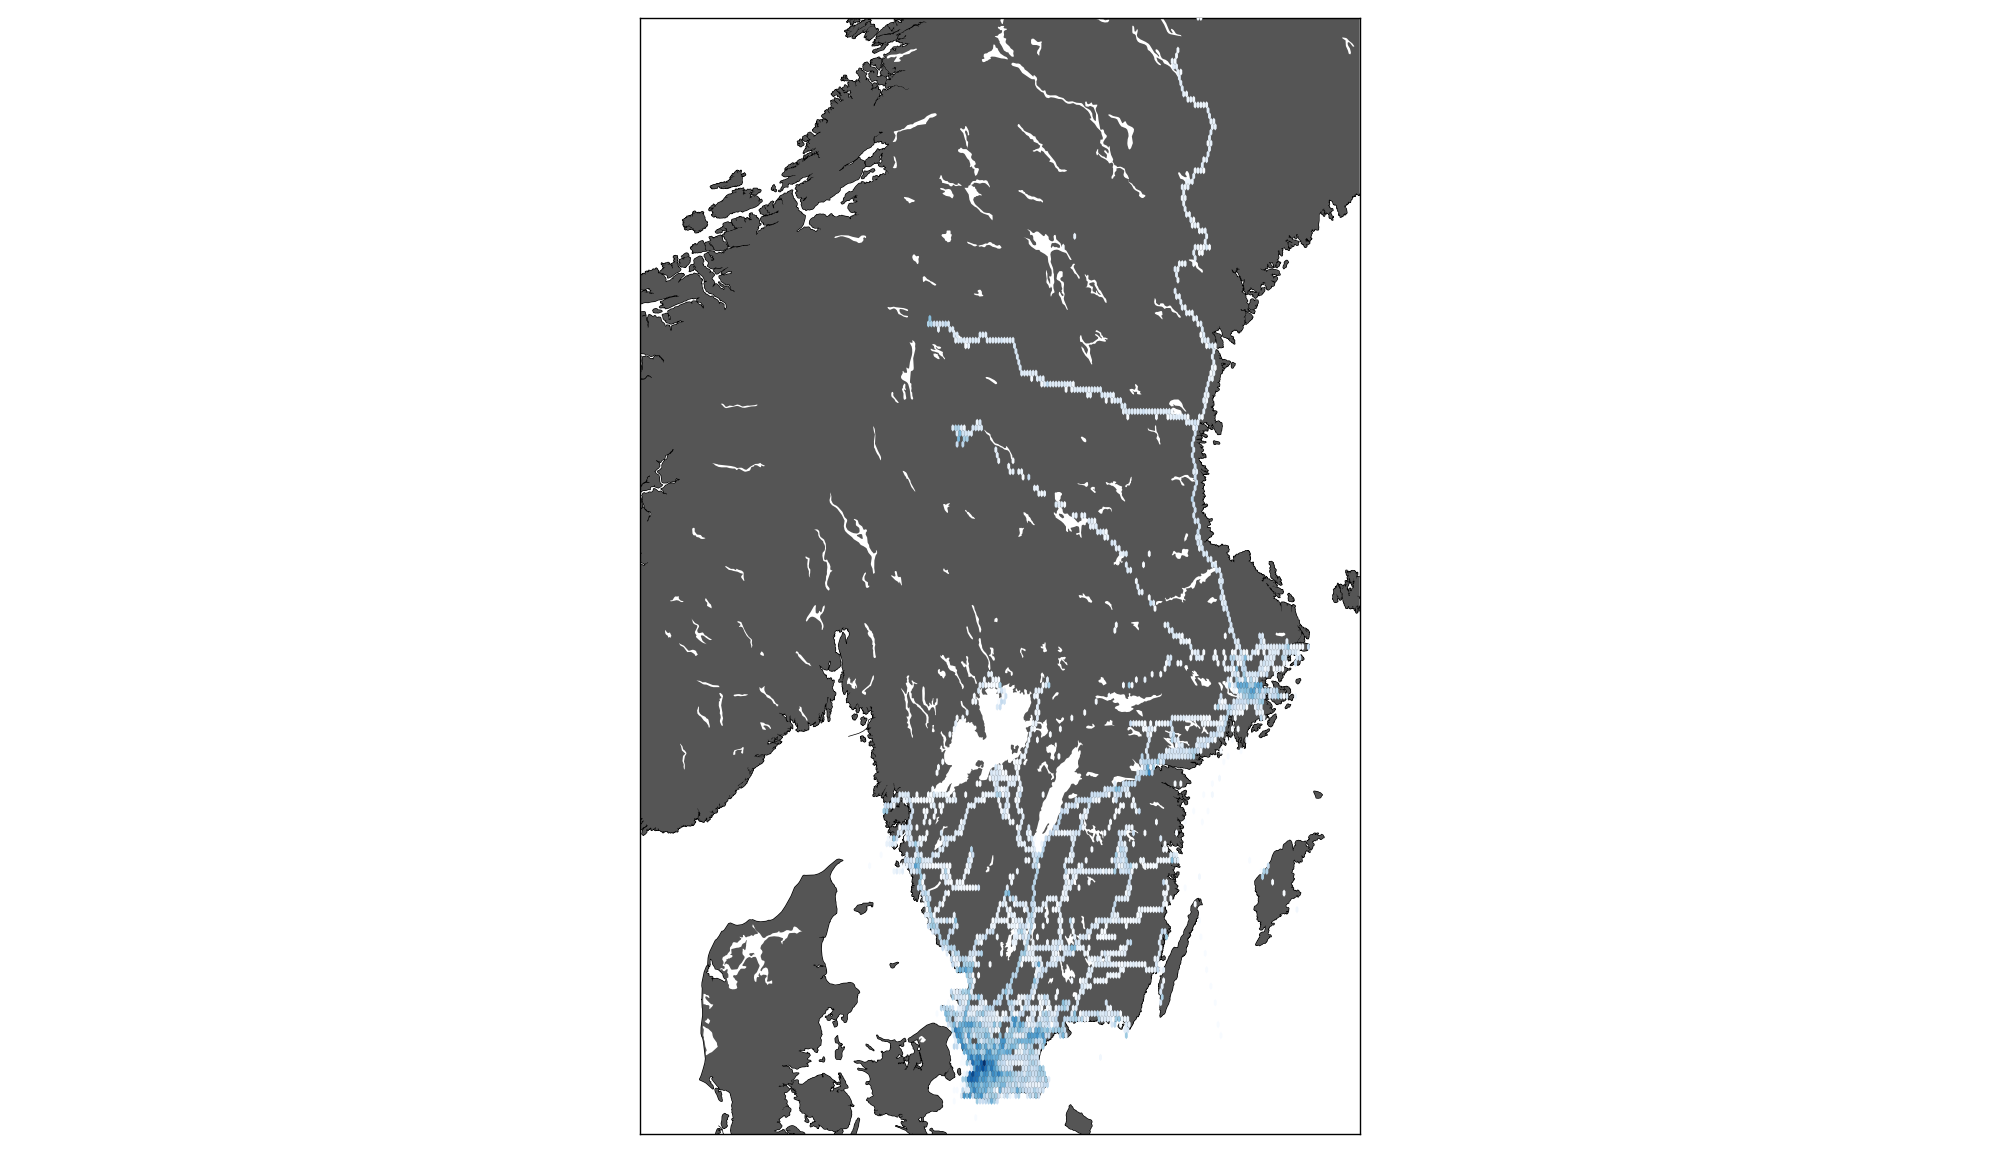
\includegraphics[scale=0.30]{all_locations_sweden}
    \caption{Location updates in Sweden, hex-binned in log scale with markers to Sony-related properties where we can see increased activity}
    \label{fig:sweden_locations_hexbin}
\end{figure}

\begin{figure}[H]
    \hspace*{-1.0cm}
    \centering
    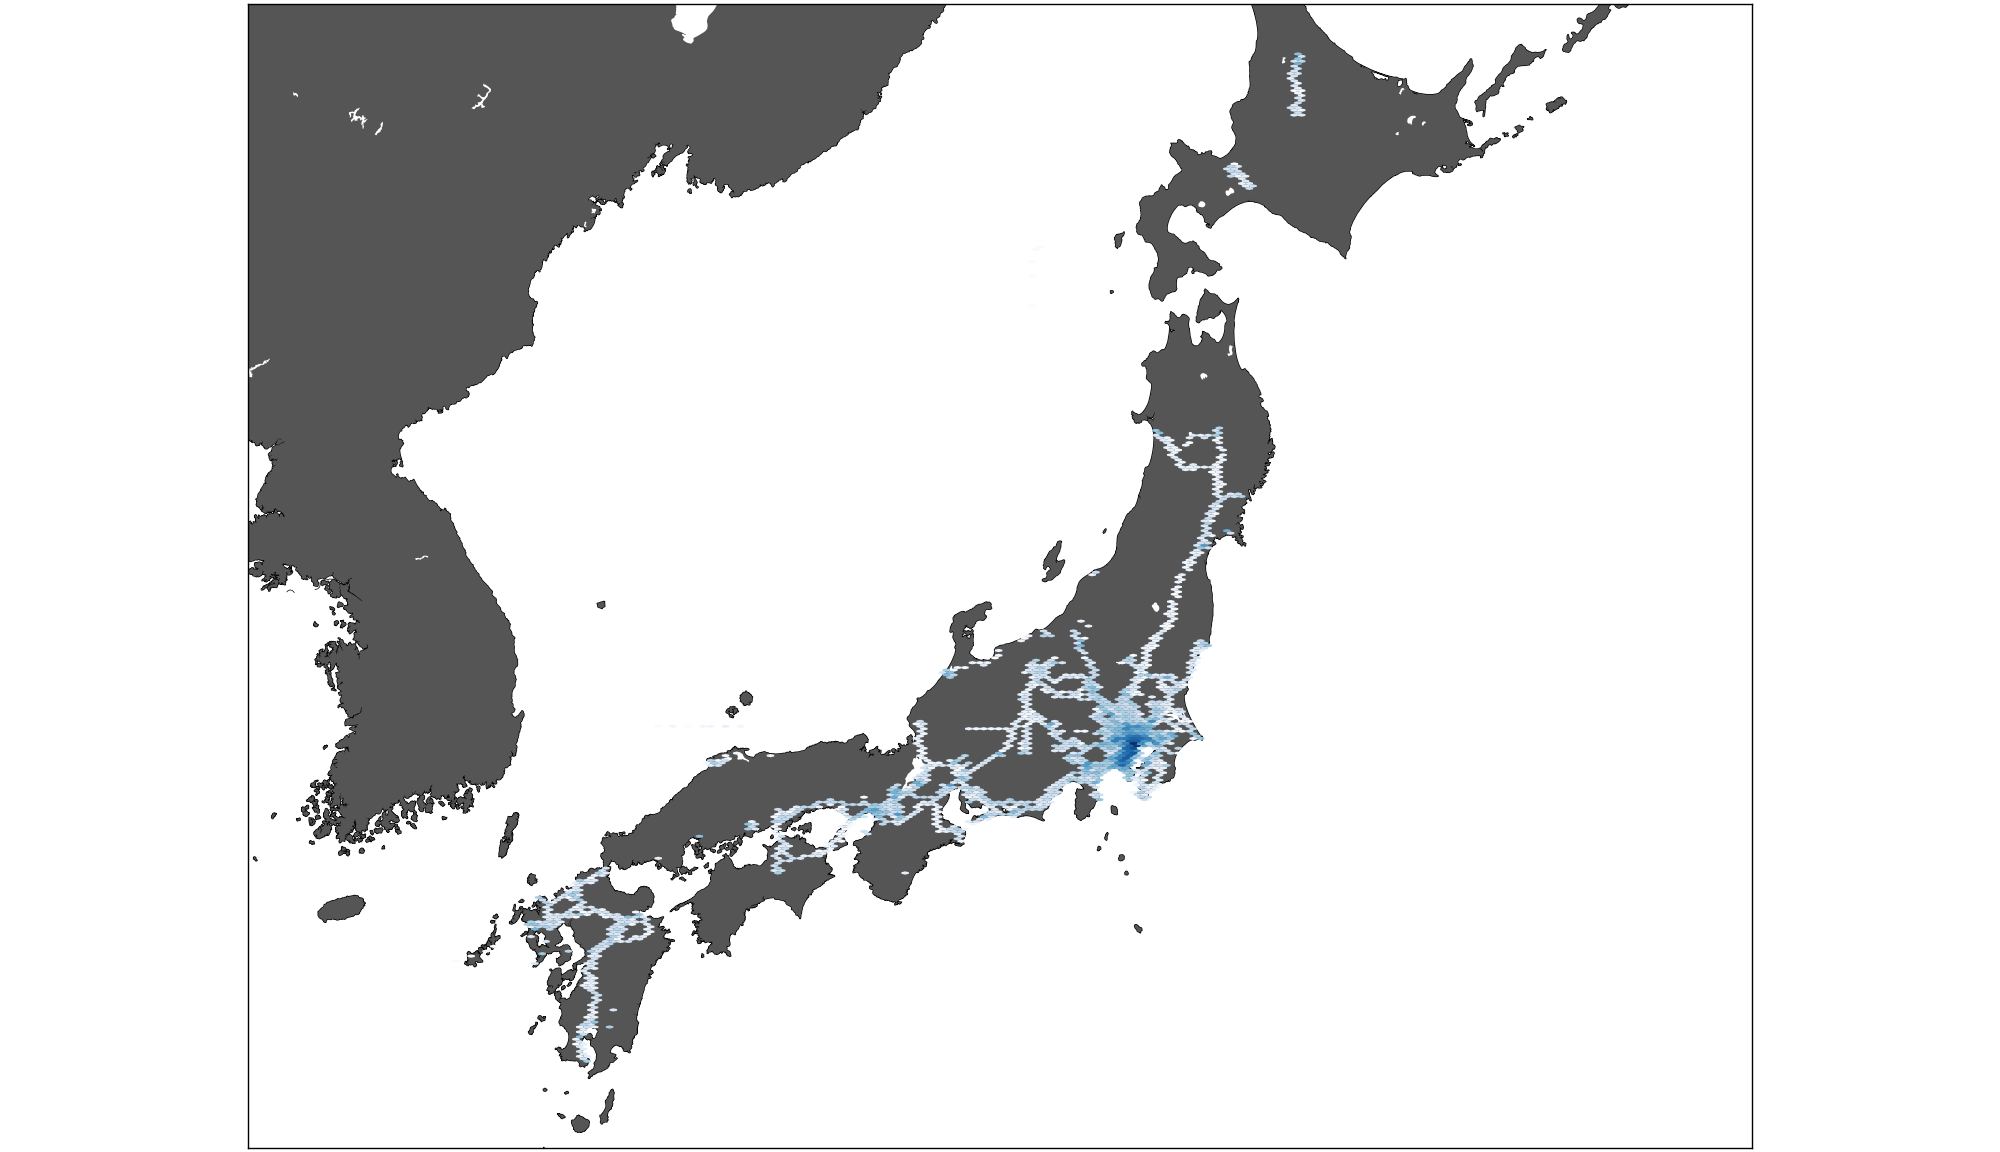
\includegraphics[scale=0.30]{all_locations_japan}
    \caption{Location updates in Japan, hex-binned in log scale with markers to Sony, Tokyo which also shows increased activity}
    \label{fig:japan_locations_hexbin}
\end{figure}
Figure \ref{fig:sweden_locations_hexbin} and Figure \ref{fig:japan_locations_hexbin} shows all location updates from Sweden and Japan for the three months plotted on a map. On Figure \ref{fig:sweden_locations_hexbin} we can see increased activity around Sony-related properties in Lund\cite{sony_headquarters_sweden_lund}, Kista\cite{sony_headquarters_sweden_kista}, and at Ericsson AB in Göteborg\cite{ericsson}. Likewise on Figure \ref{fig:japan_locations_hexbin} we can see increased activity at the Sony headquarters\cite{sony_headquarters_japan} in Tokyo. We exclude co-occurrences from these locations for our dataset as they are work-related and being at the same workplace does not constitute a valid co-occurrence.

\begin{figure}[H]
    \hspace*{-1.0cm}
    \centering
    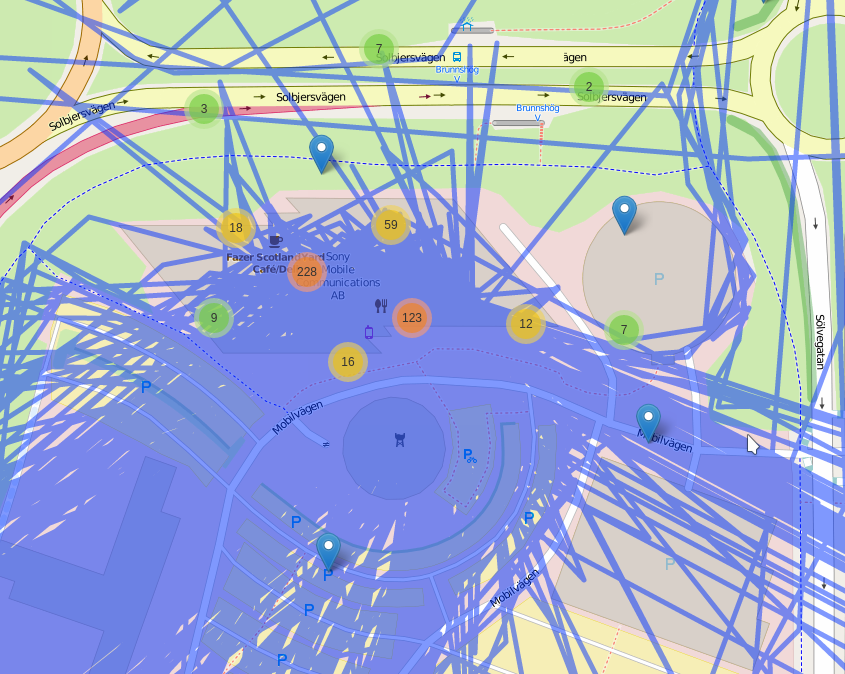
\includegraphics[scale=0.50]{user_pair_at_sony}
    \caption{User pair with high number of co-occurrences clustered for whole period at Sony perimeters, blue traces are location updates}
    \label{fig:user_pair_at_sony}
\end{figure}
Figure \ref{fig:user_pair_at_sony} shows an example of the co-occurrences visualized for a dyad in Sweden having lots of co-occurrences within the Sony perimeter. This enabled us to exclude co-occurrences from these locations from our dataset as we are looking for co-occurrences outside of the users work.


\begin{figure}[H]
    \hspace*{-1.0cm}
    \centering
    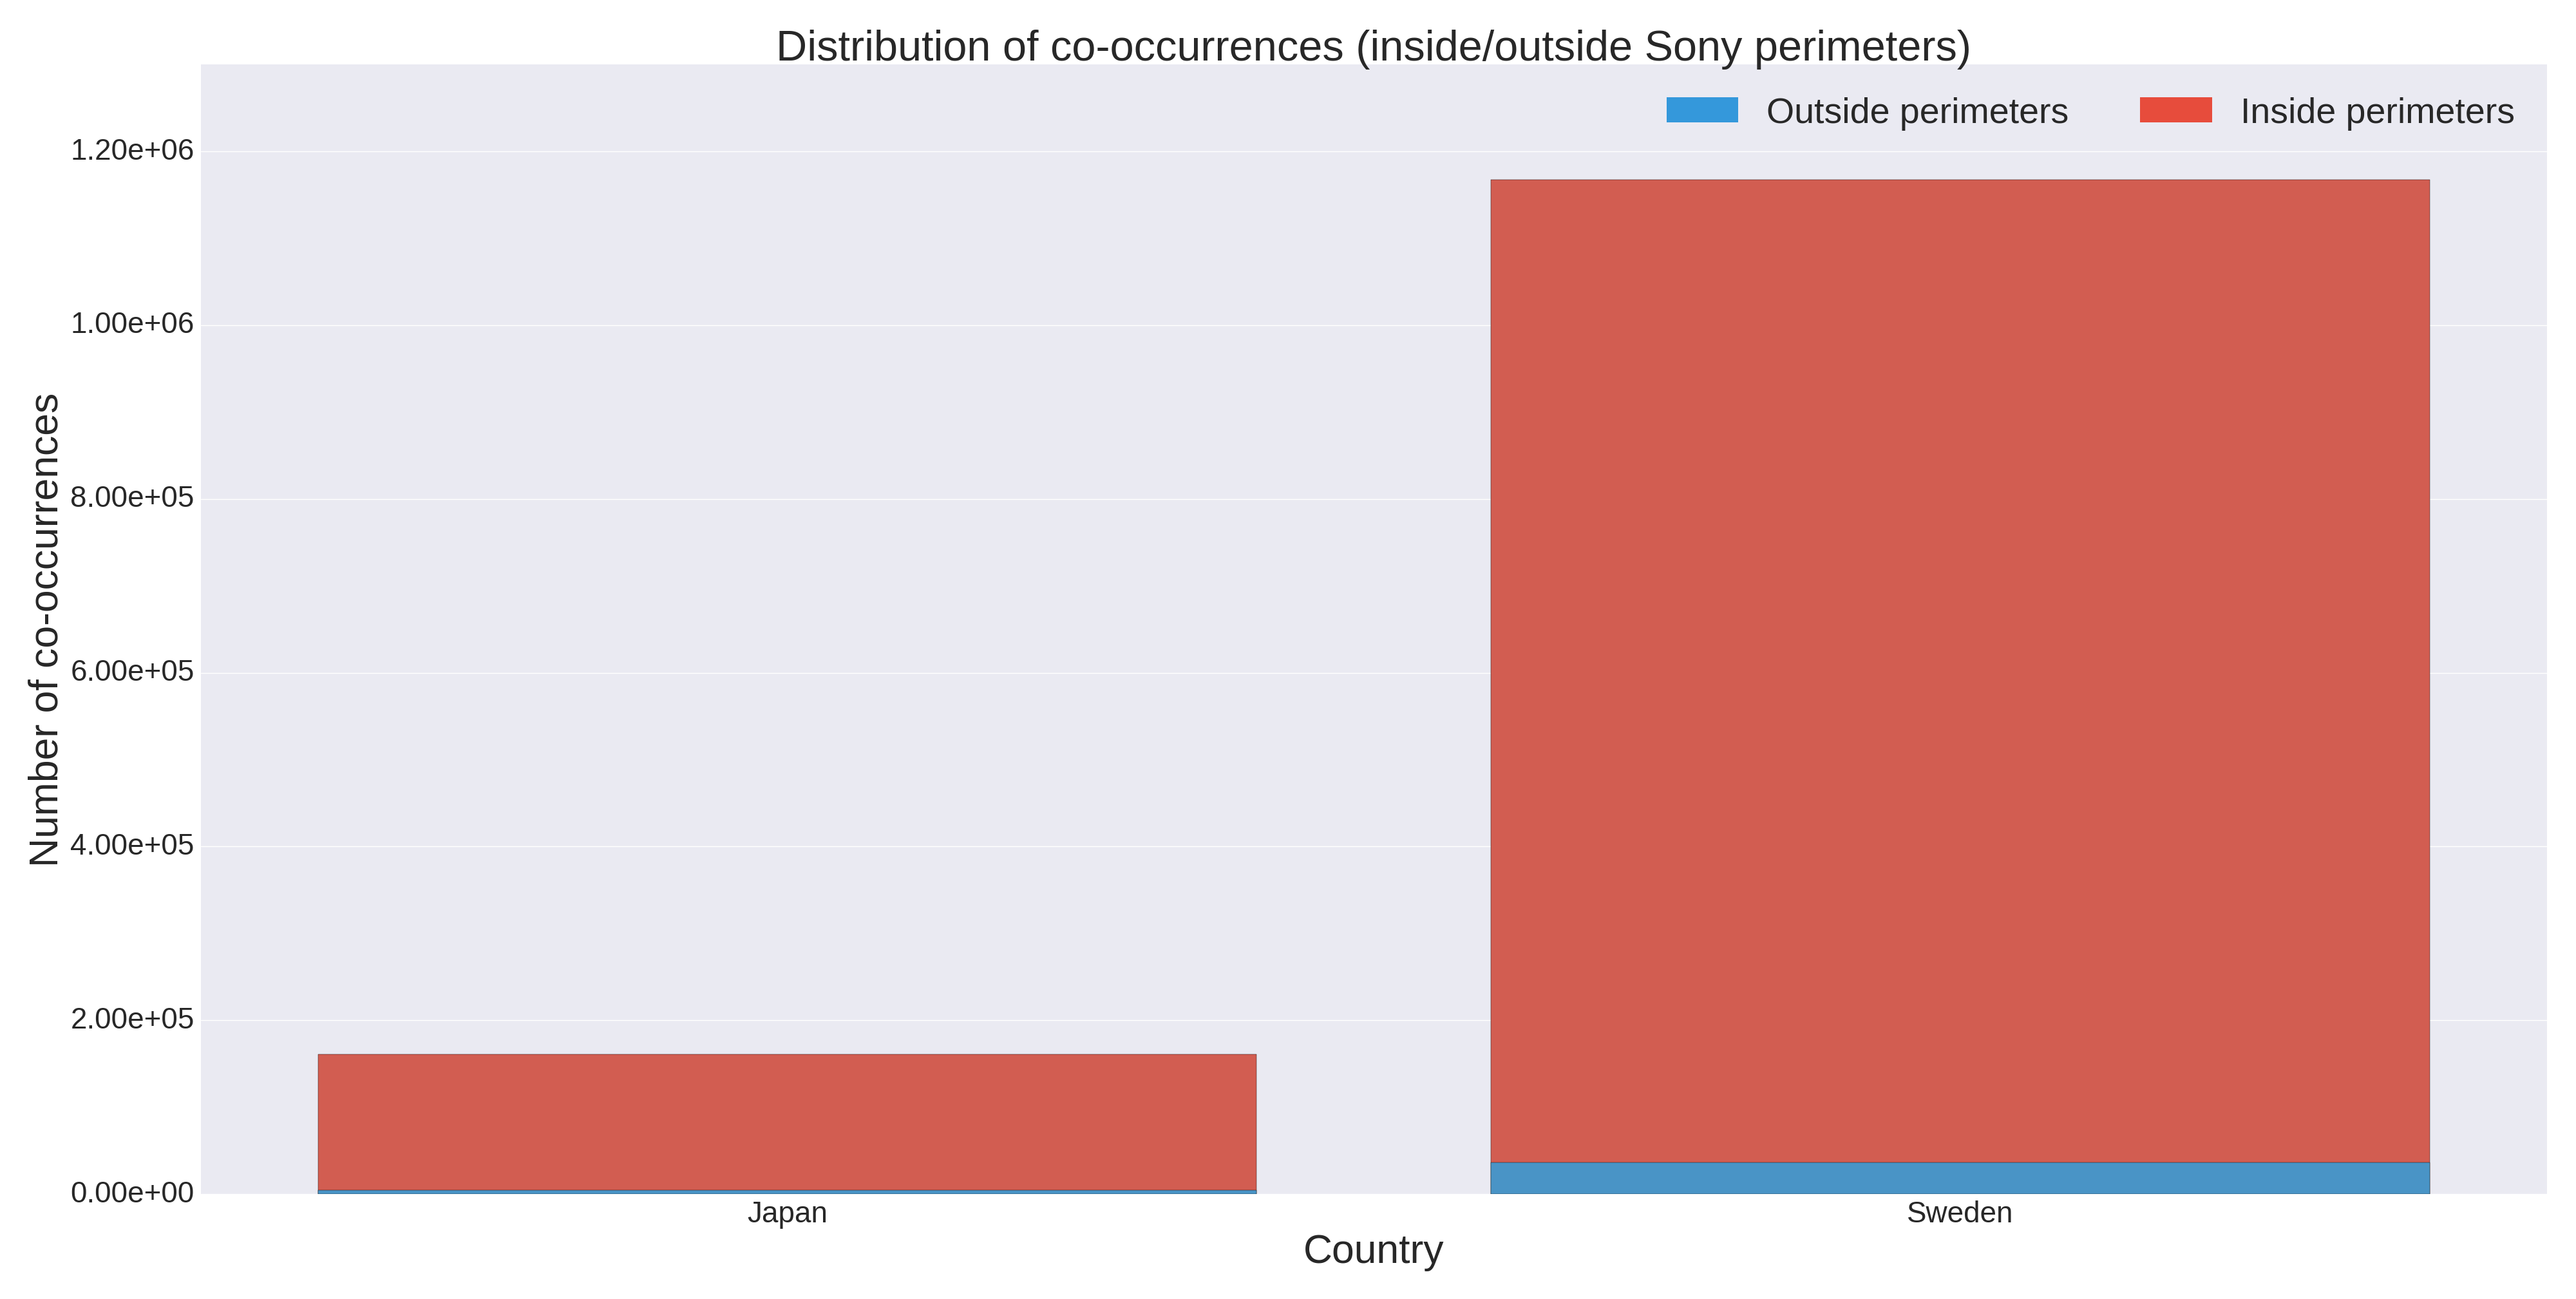
\includegraphics[scale=0.10]{stack_bar_coocs}
    \caption{Distribution of co-occurrences inside and outside Sony perimeters}
    \label{fig:dist_coocs_sony}
\end{figure}

We decided to look at just how many co-occurrences happened inside the Sony perimeter. Figure \ref{fig:dist_coocs_sony} shows the number of co-occurrences inside and outside Sony perimeters, here we see a massive amount of co-occurrences happening inside the Sony perimeters. This can pose a problem as we will only be looking at co-occurrences between users that is outside Sony perimeters.

\subsubsection{Data export to Numpy arrays}
We created scripts for exportation to numpy arrays for use in the sklearn module. The users were encoded with K values where K = number of users. The countries were encoded with K values where K = number of countries.

Each row in the dataset represents a dyad of users and the features computed for them as well as the binary label of whether they met in the next period or not.

\subsection{Preparation of Production data}
In this section we will demonstrate what we have done to prepare the production data for analysis.

The methods for binning of production data are the same as for test data\ref{ssec:binning}.

\subsubsection{Code preparation - Apache Spark}
The production data were stored on Sony's Apache Spark\cite{spark} cluster.

To manipulate the data, we converted some of our previously written code for use in \textit{RDDs} (Resilient Distributed Datasets) and \textit{Dataframes} which are fault-tolerant collections native to Spark that can be operated on in parallel.
As the size of our datasets were manageable we opted not to use the built-in machine learning library of Spark \textit{MLlib} and thus we saved the datasets in LibSVM format which enabled us to import the datasets in \textit{sci-kit learn}.

\section{Modeling}
In this subsection we will describe the model and features used for prediction.

As we do not have ground truth for friendship, we decided to use a meeting in a next period as a proxy for friendship.

We will try to answer the following question: Can we predict if people meet in a period based on their spatiotemporal patterns in a previous period.
The models and algorithms we use are implemented in \textit{scikit-learn}\cite{scikit-learn} a Python module for machine learning.

\subsection{Models}
For our work we will use two models, Logistic Regression and Random Forest. For each model we will first fit them on the complete period of 3 months and the single month of September as found in \autoref{chap:dataset}. Furthermore we will use all of the users as well as a subset of users meeting our criteria for cross-occupancy as found in \autoref{chap:dataset} of 40\% and 10\% for test and production data respectively. For the datasets we will use an outer loop of 2-fold cross-validation and an inner loop of randomized search. We choose randomized search over grid search because of the efficiency in computation time. We will use ROC AUC as the score function for the randomized search.


\subsubsection{Logistic Regression}
The Logistic Regression model will be used as the baseline model. It will be fit on only one feature, whether or not people have had two co-occurrences in distinct spatial bins. We will compare the predictive strength of just that one feature to several different features fitted to a Random Forest model.

\subsubsection{Random Forest}
The random forest is an \textit{ensemble learning} classifier which means it fits several models to obtain better predictive performance than just a single model would achieve. In the case of the random forest it fits several decision trees. Each decision tree is fitted with a random sample with replacement of the training data, a technique called \textit{bagging}. Furthermore it uses a random subset of features. The predicted class will then be the \textit{mode} of predictions of the decision trees.

In the following sections we will describe the different features which our models are fitted on.

\subsection{Spatial Features}

\subsubsection{Specificity}
The total number of co-occurrences between two users divided by the sum of the two users location updates. Feature ID: \textit{14}

\subsubsection{Number of co-occurrences}
The total number of co-occurrences between users. Feature ID: \textit{7}.

\subsubsection{Diversity of a co-occurrence}
We use the diversity measure taken from the papers of Shahabi and Pham\cite{iRWRfSD}\cite{AEBMtISSfSD}.
Diversity is a measure of how important the spatial locations of the co-occurrences between a dyad is, given how many times they appear.
The diversity measure uses the Shannon entropy, which holds the amount of location information in the co-occurrences of each dyad and yields a higher value with more locations and a more equal distribution of updates for each location.
Feature ID: \textit{2}.
The Shannon entropy is defined by Equation \ref{eq:shannon_entropy}
\begin{equation}
\label{eq:shannon_entropy}
H^S_{ij}=-\sum\limits_{l}P^l_{ij} \log P^l_{ij}= -\sum\limits_{l,c_ij,l\neq 0}\frac{c_{ij,l}}{f_{ij}}\log \frac{c_{ij,l}}{f_{ij}}
\end{equation}
where $f_{ij}$, the \textit{frequency}, is the total number of co-occurrences between user $i$ and user $j$, and $c_{ij,l}$, the \textit{local frequency}, is the total number of co-occurrences between user $i$ and $j$ at location $l$.
From this the diversity is defined by taking the exponential function of the entropy defined in Equation \ref{eq:diversity}:
\begin{equation}
\label{eq:diversity}
D^s_{ij} = exp(H^S_{ij})
\end{equation}

\subsubsection{Two unique co-occurrences}
If the user \textit{i} and \textit{j} has at least two unique co-occurrences in terms of spatial bins. This feature is only used for the baseline model. Feature ID: \textit{0}.

\subsubsection{Unique co-occurrences}
The number of unique co-occurrences in terms of spatial bins between two users \textit{i} and \textit{j}. Feature ID: \textit{3}.

\subsubsection{Weighted frequency}
We use the weighted frequency measure taken from the papers of Shahabi and Pham\cite{iRWRfSD}\cite{AEBMtISSfSD}.
Weighted frequency is a measure of how important the co-occurrences at non-popular places are.
It uses the Shannon entropy for a location, where a more crowded place yields a higher entropy.
Feature ID: \textit{4}.
The weighed frequency is defined by Equation \ref{eq:weighted_frequency}
\begin{equation}
\label{eq:weighted_frequency}
F_{ij}=\sum\limits_{l}c_{ij,l} \times \exp(-H_l)
\end{equation}
where $H_l$ is the entropy for location \textit{l} defined in Equation \ref{eq:location_entropy}
\begin{equation}
\label{eq:location_entropy}
H_l = \sum\limits_{u, P_{u,l}\neq0} P_{u,l}\log P_{u,l}
\end{equation}
where $P_{u,l}$ is the probability that a location update from location \textit{l} belongs to user \textit{u}.

\subsubsection{Co-occurrences weighted with respect to each location}
We use the weighted co-occurrences measure proposed in the master's thesis of Sapieżyński\cite{IMM2013-06556}.
The co-occurrences between users \textit{i} and \textit{j} are weighted by how many other people are present in the same spatial bin and time bin.
Feature ID: \textit{5}.

\subsubsection{Common travels}
We use the common travels measure proposed in the master's thesis of Sapieżyński\cite{IMM2013-06556}.
The number of common travels between two users. Common travels are defined when user \textit{i} and user \textit{j} co-occur in consecutive time-bins with each spatial bin being different than the previous one. Feature ID: \textit{6}.

\subsubsection{Mutual co-occurrences}
Number of mutual co-occurrences, the mutual co-occurrences for user \textit{i} and \textit{j} will be the number of users, with whom they share co-occurrences. Feature ID:\textit{8}.

\subsection{Homophily Features}
Based on the work by McPherson et al.\cite{mcpherson2001birds} on homophily in personal networks, we have tried to create several features based on homophily between users.

\subsubsection{Within 6 years of age}
McPherson et al.\cite{mcpherson2001birds} found that age homophily is a strong dimension with respect to close friendship.
This feature explains if a dyad of users are within 6 years of age of each other.
Because this feature is categorical, we apply one-hot-encoding which converts it to three binary features, NO, YES, N/A. Feature ID: \textit{13,14,15}

\subsubsection{Same gender}
This feature explains if a dyad of users share the same gender. 
Because this feature is categorical, we apply one-hot-encoding which converts it to three binary features, NO, YES, N/A.Feature ID: \textit{16,17,18}

\subsubsection{App usage similarity}
The Jaccard index is a measure used in comparing the similarity of sample sets. We extract what apps two users have \textit{i} and \textit{j} used in the period and compute the similarity between them using the Jaccard index. Feature ID:\textit{9}.
The Jaccard index is defined in Equation \ref{eq:jaccard_index}
\begin{equation}
\label{eq:jaccard_index}
J(A_i,A_j) = \frac{ |A_i \cap A_j| }{ |A_i \cup A_j | }
\end{equation}
where $A_i$ is the set of apps used by user $i$ and $A_j$ is the set of apps used by user $j$. If $A_i$ and $A_j$ are empty sets we define $J(A_i, A_j) = 1$

\subsection{Temporal features}
In this section we have features related to the time of the co-occurrences.

\subsubsection{Timely arrival and leaving}
We use the timely arrival and leaving measure proposed in the master's thesis of Sapieżyński\cite{IMM2013-06556}.
Sapieżyński argued that two persons arriving or leaving a location synchronously could be more indicative of friendship than them arriving or leaving non-synchronously. If for every co-occurrence one of the persons remains in the antecedent or subsequent time bin, the co-occurrence is non-synchronously arrived or left at.
Feature ID: \textit{1}.

\subsubsection{Number of weekends}
How many co-occurrences between two users happened in the weekend, defined as either a Friday after 18:00, a Saturday or a Sunday.
Feature ID: \textit{11}.

\subsubsection{Number of evenings}
How many co-occurrences between two users happened after 18:00.
Feature ID: \textit{10}.

\subsection{Overview}
\label{ssec:overview}
In this section we will give an overview of which model we will fit on which data. As Logistic Regression works as our baseline and Random Forest will be compared up against Logistic Regression, we will end up with pairs of Logistic Regression and Random Forest. We will come back to this later. \\
First we will show which features the two models (Logistic Regression and Random Forest) use on which dataset. 
\begin{table}[H]
\centering
\begin{tabular}{|c|c|c|c|l|c|c|}
\hline
\multirow{2}{*}{Feature ID} & \multirow{2}{*}{Feature name} & \multicolumn{3}{c|}{Test data}             & \multicolumn{2}{c|}{Production data} \\ \cline{3-7} 
                            &                               & T-LR         & \multicolumn{2}{c|}{T-RF}   & P-LR              & P-RF             \\ \hline
0                           & Two unique co-occurrences     & \cmark       & \multicolumn{2}{c|}{}       & \cmark            &                  \\ \hline
1                           & Timely arrival and leaving    &              & \multicolumn{2}{c|}{\cmark} &                   &                  \\ \hline
2                           & Diversity                     &              & \multicolumn{2}{c|}{\cmark} &                   & \cmark           \\ \hline
3                           & Unique co-occurrences         &              & \multicolumn{2}{c|}{\cmark} &                   & \cmark           \\ \hline
4                           & Weighted frequency            &              & \multicolumn{2}{c|}{\cmark} &                   & \cmark           \\ \hline
5                           & Co-occurrences weighted       &              & \multicolumn{2}{c|}{\cmark} &                   & \cmark           \\ \hline
6                           & Common travels                &              & \multicolumn{2}{c|}{\cmark} &                   &                  \\ \hline
7                           & Number of co-occurrences      &              & \multicolumn{2}{c|}{\cmark} &                   & \cmark           \\ \hline
8                           & Mutual co-occurrences         &              & \multicolumn{2}{c|}{\cmark} &                   & \cmark           \\ \hline
9                           & App usage similarity          &              & \multicolumn{2}{c|}{\cmark} &                   &                  \\ \hline
10                          & Number of evenings            &              & \multicolumn{2}{c|}{\cmark} &                   & \cmark           \\ \hline
11                          & Number of weekends            &              & \multicolumn{2}{c|}{\cmark} &                   & \cmark           \\ \hline
12                          & Specificity                   &              & \multicolumn{2}{c|}{\cmark} &                   & \cmark           \\ \hline
13,14,15                    & Within 6 years of age [NO, YES, N/A]   &         & \multicolumn{2}{c|}{\cmark} &                   &                  \\ \hline
16,17,18                    & Same gender [NO, YES, N/A]                  &              & \multicolumn{2}{c|}{\cmark} &                   &                  \\ \hline

\end{tabular}
\caption{Overview of the features used by each model in Test data and Production data. T-LR = Test data Logistic Regression, T-RF = Test data Random Forest, P-LR = Production data Logistic Regression, P-RF = Production data Random Forest}
\label{tab:model_overview}
\end{table}
Table \ref{tab:model_overview} give an overview, where we have a Logistic Regression and Random Forest for both Test data and Production data. Both Logistic Regressions (T-LR \& P-LR) will only use one feature, as earlier explained, as it will be used as the baseline. The Random Forest models (T-RF \& P-RF) will be using all of the features for Test data and some of the features for Production data. See \autoref{chap:discussion} on why we only used some of the features.   


Table \ref{tab:model_delimitation} shows which sub-period and data delimitations each of the models from Table \ref{tab:model_overview} (T-LR, T-RF, P-LR, P-RF) uses. 

\begin{table}[H]
\centering
\begin{tabular}{|l|c|c|c|c|c|}\hline
\diaghead{\theadfont Diag ColumnmnHead II}%
{Data\\delimitation}{Model}&
\thead{T-LR}&\thead{T-RF}& \thead{P-LR}&\thead{P-RF}\\    \hline
\thead{All three month} & \cmark & \cmark &  & \\    \hline
\thead{September\\All users} &  &  & \cmark & \cmark \\    \hline
\thead{September \\Users with \\40\% cross-occupancy} & \cmark & \cmark &  & \\    \hline
\thead{September \\Users with \\10\% cross-occupancy} &  &  & \cmark & \cmark \\    \hline
\end{tabular}
\caption{Overview of which models from Table \ref{tab:model_overview} (T-LR, T-RF, P-LR, P-RF) that uses which sub-period and other delimitations}
\label{tab:model_delimitation}
\end{table}

As Table \ref{tab:model_delimitation} shows, we end up with four model-pairs. Each represented as a row in the table (exclusive table header): 
\begin{itemize}
\item All three month (September, October, November) for all users\\ \textbf{Name ID: TP-1}
\item For September for all users\\ \textbf{Name ID: PP-1}
\item For September for users with 40\% cross-occupancy\\ \textbf{Name ID: TP-2}
\item For September for users with 10\% cross-occupancy\\ \textbf{Name ID: PP-2}
\end{itemize}

For each of the pairs (TP-1, PP-1, TP-2, PP-2), the Random Forest will be compared with the baseline, the Logistic Regression. 

